
Let \textbf{M} be the midpoint of two points \textbf{A}=\myvec{3\\4} and \textbf{B}=\myvec{-1\\2}.
\begin{align}
    \vec{M}=\frac{\vec{A}+\vec{B}}{2}=\frac{1}{2}\myvec{2\\6}\\
    \implies\vec{M}=\myvec{1\\3}\nonumber
\end{align}
The direction vector of line AB is
\begin{align}
    \myvec{-1\\2}-\myvec{3\\4}=\myvec{-4\\-2}
\end{align}
The direction vector of line AB is normal vector of right bisector. Then
\begin{align}
    \vec{n}=\myvec{-4\\-2}
\end{align}
The equation of line in terms of normal vector is then obtained as
\begin{align}
    \vec{n}^T(\vec{x}-\vec{M})=0\\
    \implies\left(\begin{array}{cc}-4 & -2\end{array}\right)\left(\vec{x}-\myvec{1\\3}\right) = 0\\
    \implies\left(\begin{array}{cc}-4 & -2\end{array}\right)\vec{x} = -10\\
    \implies\left(\begin{array}{cc}2 & 1\end{array}\right)\vec{x} = 5
\end{align}
We got equation of the right bisector of line segment joining points \textbf{A} and \textbf{B}. The line also passes through point \textbf{M}.

See Fig.~\ref{fig:sol_line_plane_41_figure1} for plot of line segment and right bisector.
\begin{figure}[ht!]
    \centering
    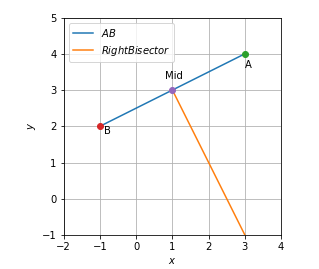
\includegraphics[width=\columnwidth]{./solutions/line_plane/41/Figure_1}
    \caption{Right bisector of line AB}
    \label{fig:sol_line_plane_41_figure1}
\end{figure}
